\chapter{Fundamentos teóricos}
\pagenumbering{arabic}

\section{Redes neuronales recurrentes de tiempo continuo (CTRNN)}
En contraste con las redes neuronales feed-forward, las cuales soportan únicamente comportamientos
reactivos, en las Redes Neuronales Recurrentes de Tiempo Continuo (CTRNN) \cite{BeerRD}
pueden existir ciclos en su estructura y la activación de sus neuronas es asíncrona y multiescalada
en el tiempo. Este tipo de redes neuronales también facilita describir el agente como un
sistema dinámico acoplado al entorno en el que está ubicado, ya que está demostrado que son el
modelo más simple de red neuronal dinámica continua no lineal \cite{FunaYNaka}
Además, la interpretación neurobiológica de las CTRNN ha sido demostrada y puede consultarse
en \cite{BeerRD}.

\subsubsection{Descripción matemática de una CTRNN}
Las CTRNN están formadas por neuronas cuyo comportamiento se describe en las ecuaciones \ref{eq:funcionCTRNN} y \ref{eq:funcionSIGMOIDE}
\begin{equation} \label{eq:funcionCTRNN}
	\dot{y_{i}}= \frac{1}{\tau_{i}} * \left ( -y_{i}+\sum_{j=1}^{N}w_{ji}*\sigma \left ( y_{j} + \theta _{j} \right ) + I_{i} \right ) \qquad i =1,2,...,N
\end{equation}
\begin{equation} \label{eq:funcionSIGMOIDE}
	\sigma (x)=\frac{1}{1+e^{-x}}
\end{equation}
donde $y_{i}$ es el estado de la neurona, $w_{ji}$ es el peso de la conexión entre las neuronas i y j,
$\theta$ es el término bias, I representa una entrada externa y $\tau$ hace que cada una de las neuronas
dependa del tiempo, ya que para diferentes valores la caída del nivel de activación de la neurona
es más rápida o lenta. En la fórmula \ref{eq:funcionCTRNN} la velocidad de actualización de la red neuronal debe ser
notablemente mayor (el intervalo entre dos actualizaciones será menor) que el valor de $\tau$ para no
obtener comportamientos no deseados.

\subsubsection{Valores de activación y de salida de la neurona de una CTRNN}
Para poder entender cómo deben interpretarse la activación y la salida de una CTRNN, se va
a utilizar como ejemplo una CTRNN formada por una única neurona autoconectada como la de la figura \ref{fig:figuraCTRNNBasica}.
El valor de salida o de una neurona será un valor real entre 0 y 1 obtenido al aplicar la función
sigmoide (ecuación \ref{eq:funcionSIGMOIDE}) a la suma del estado actual y de la neurona con su valor bias $\theta$, tal y
como puede verse en la figura \ref{fig:figuraCTRNNBasica}.
\begin{figure}[H]
    \centering
    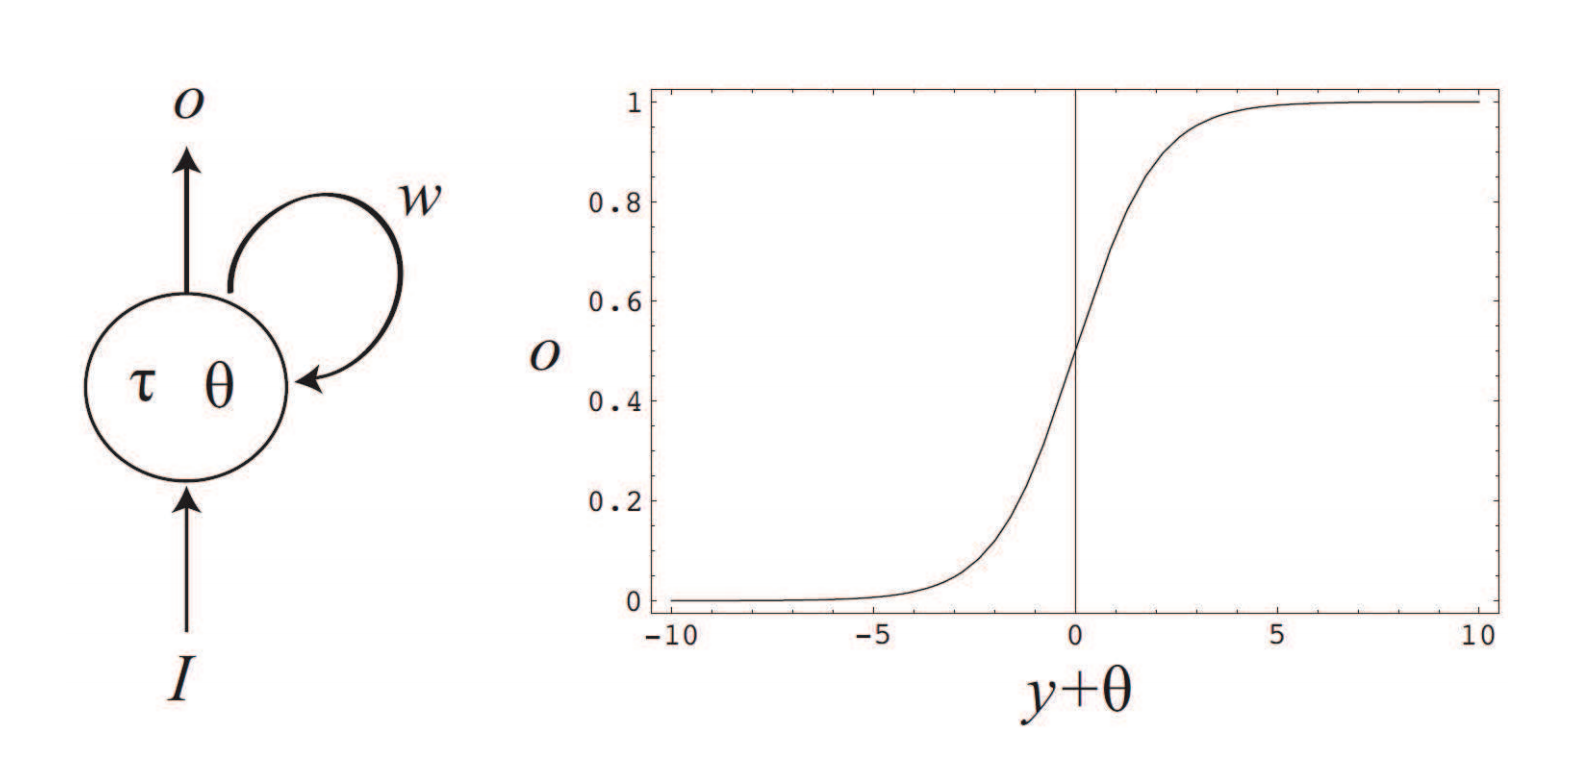
\includegraphics[width=0.8\textwidth,height=6cm]{Imagenes/CTRNNBasica}
    \caption{Valor de salida de una CTRNN. \textbf{Izquierda:} Un nodo autoconectado. \textbf{Derecha:} Función sigmoide aplicada para calcular la salida de una neurona.}
    \label{fig:figuraCTRNNBasica}
\end{figure}

En cuanto al valor de activación, a diferencia de una red neuronal feed-forward, la cual realiza
un mapeo directo entre entrada y salida de la red, el comportamiento de una CTRNN corresponde
al de un sistema dinámico \cite{BeerRD}, por lo que el valor de activación de la neurona convergerá
a un punto de equilibrio. Para el análisis de las dinámicas del sistema formado por el agente
controlado por la CTRNN y el entorno, se analizarán sus diagramas de bifurcación, los cuales
muestran todos los puntos de equilibrio para la activación de las neuronas de la red.

\section{Homeostasis}
A pesar de que la homeostasis es una propiedad biológica, es posible representar un sistema lógico que se comporte de forma similar a como
sistemas vivos con estas propiedades lo harían\cite{Hywel}.

Un \textit{Homeostato}, es un sistema artificial que presenta porpiedades de homeostasis. El Homeostato desarrolado por Ashby era un aparato
electromagnético mientras que el que va a ser utilizado es un componente implementado computacionalmente.

Un Homeostato es un sistema de $N$ neuronas completamente interconectadas entre si. Cada neurona recibe $N$ entradas, de si misma y del resto de neuronas,
dependientes del peso de la fuerza de conexión de las uniones entre ellas (ver Figura \ref{fig:figuraHomeostatSchema}).

\begin{figure}[!h]
    \centering
    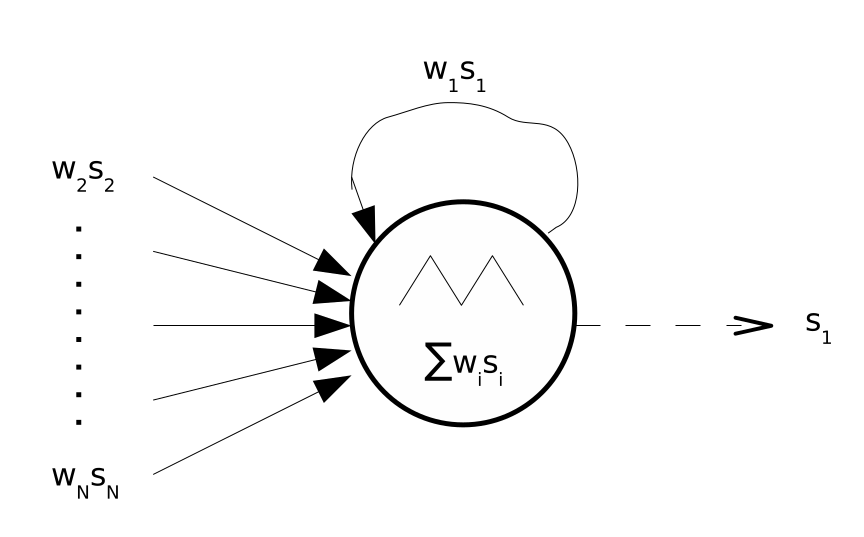
\includegraphics[width=0.6\textwidth,height=5cm]{Imagenes/HomeostatSchema}
    \caption{Esquema de un Homeostato individual. La unidad recibe las entradas del resto de unidades ($w_{i}s_{i}$) y de si misma ($w_{1}s_{1}$). La salida $s_{1}$ es una función lineal por partes
		de la suma ponderada de las entradas.)}
    \label{fig:figuraHomeostatSchema}
\end{figure}

\begin{figure}[!h]
    \centering
    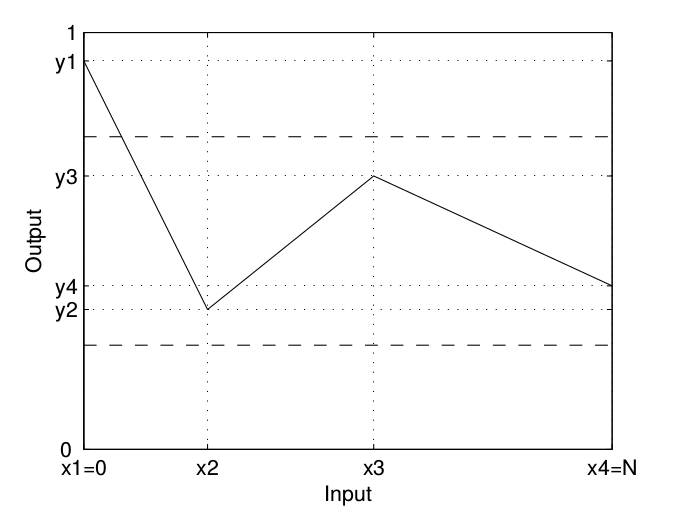
\includegraphics[width=0.6\textwidth,height=6cm]{Imagenes/HomeostatTransfer}
    \caption{Ejemplo de función de transferencia de una unidad Homeostat. La función es lineal por partes con puntos en ($x_{1},j_{1}$),...,($x_{p},y_{p}$) donde $x_{1}$ = 0 y $x_{p}$ = $N$, para todas las
		unidades en una red de $N$ unidades. Las lineas discontinuas representan el rango homeostatico de la red.}
    \label{fig:homeostatTransferFunction}
\end{figure}

La suma ponderada $I$ (ver equación \ref{eq:sumaPonderadaHomeostat}) de las entradas de una unidad determina su salida $s$, tal y como esta especificado por la función linear de transferencia por
partes $F$ (equación \ref{eq:ecuPartesHomeostat} y figura \ref{fig:homeostatTransferFunction}).

\begin{equation} \label{eq:sumaPonderadaHomeostat}
	I = \sum_{i}^{N}w_{i}s_{i}
\end{equation}

\begin{equation} \label{eq:ecuPartesHomeostat}
	s = F(I)=\begin{cases}
y_{1}+(y_{2}-y_{1})(\frac{I-x_{1}}{x_{2}-x_{1}}) & \text{ : }\quad x_{1} \leq I < x_{2} \\
y_{2}+(y_{3}-y_{2})(\frac{I-x_{2}}{x_{3}-x_{2}}) & \text{ : }\quad x_{2} \leq I < x_{3} \\
y_{3}+(y_{4}-y_{3})(\frac{I-x_{3}}{x_{4}-x_{3}}) & \text{ : }\quad x_{3} \leq I \leq  x_{4} \\
\end{cases}
\end{equation}

Al inicializar la red, los pesos de las conexiones se aleatorizan a partir de una distribución uniforme de rango apropiado. El rango objetivo (o rango límite) $R = [0.5 - \delta, 0.5 + \delta]$ es
especificado para la salida, donde $\delta$ determina la rigidez de la restricción homeostática. Si $s \in R$ la unidad es homeostática. Si $s \notin R$ significa que la homeostasis se ha perdido
y se activan los mecanismos de cambio adaptativo.

Hay dos mecanismos de cambio adaptivo que se aplican a los parametros de las unidades no homeostáticas. El primer mecanismo asigna valores aleatorios a los pesos de las conexiones aferentes a la unidad (equación \ref{eq:aferenteEQ}).
El segundo mecanismo asigna nuevos valores aleatorios a los parametros que indican las coordenadas de la función de transferencia de la unidad (equación \ref{eq:transferEQ}). Los rangos de estas reasignaciones son los mismos utilizados
en la inicialización. Donde $rand(a,b)$ representa a la función que devuelve un número real aleatorio obtenido de una distribución uniforme en el rango $[a,b]$.

\begin{equation} \label{eq:aferenteEQ}
	\text{\textit{IF}} \quad (s \notin R) \quad \text{\textit{THEN}} \quad [w= \text{\textit{rand}}(0.00, 1.00) \quad \forall w \in \left \{ w_{1},...,w_{N} \right \}]
\end{equation}

\begin{equation} \label{eq:transferEQ}
	\begin{aligned}
	 \text{\textit{IF}} \quad (s \notin R) \quad \text{\textit{THEN}} \quad [x= \text{\textit{rand}}(0.00, N) \quad \forall x \in \left \{ x_{2},...,x_{p-1} \right \}]& \\
	 \qquad \qquad \qquad \,\quad  \text{\textit{AND}} \quad [y= \text{\textit{rand}}(0.00, 1.00) \quad \forall y \in \left \{ y_{1},...,y_{p} \right \}]& \\
 \end{aligned}
\end{equation}


\section{Algoritmo genético}
Los algoritmos genéticos son un tipo de algoritmos de optimización, lo que quiere decir que se utilizan para
obtener la solución o soluciones óptimas de un problema computacional\cite{JennaCarr}.

Estos algoritmos representan una rama dentro del campo conocido como ''Computación evolutiva". En ella, se
imitan los procesos biológicos de reproducción y selección natural con el fin de encontrar la mejor solución al
problema para el que son creados. Al igual que en la evolución, muchos de los procesos de un algoritmo genético son
aleatorios, aunque las técnicas de optimización permiten limitar el nivel de aleatoriedad y adaptar el control sobre
el algoritmo que se considere necesario.

Este tipo de algoritmos permiten encontrar soluciones a problemas que otros algoritmos de optimización no pueden calcular
por falta de continuidad, derivabilidad, linealidad u otras características.

\subsection{Componentes, estructura y terminología}
Dado que los algoritmos genéticos están diseñados para simular procesos biológicos, gran parte de su terminología ha sido tomado
prestada de la biología. A pesar de ello, las entidades a las que esta terminología se refieren en el entorno de los algoritmos genéticos
son mucho más simples que sus equivalentes biológicos. Los componentes básicos de prácticamente todos los algoritmos genéticos son:

\begin{itemize}
	\item{Una función \textbf{fitness} para la optimización}
	\item{Una \textbf{población} de \textbf{cromosomas}}
	\item{Una función de \textbf{selección} para elegir los cromosomas que van a reproducirse}
	\item{Una función de \textbf{recombinación} (o \textit{crossover}) para la producción de la siguiente generación de cromosomas}
	\item{Una función de \textbf{mutación} para aleatorizar algunos cromosomas de la nueva población}
\end{itemize}

La \textit{función fitness} es la función que el algoritmo está tratando de optimizar. La palabra "fitness" se toma prestada de la teoría evolutiva.
Se utiliza porque la función de fitness testea y valora como de buena (como de "\textit{fit}") es cada solución potencial del problema. El término
\textit{cromosoma} hace referencia al valor o valores numéricos que representan posibles soluciones candidatas al problema que se está intentando resolver.
Cada cromosoma está formado por una lista de parámetros, llamados \textit{genes}. Al conjunto de cromosomas que van a evaluarse como posibles candidatos a solución
del problema se le llama \textit{población}. Antiguamente los cromosomas eran codificados como listas de unos y ceros (codificación binaria), sin embargo, actualmente la computación
moderna permite codificar los cromosomas como números reales u otros objetos.

\begin{figure}[H]
    \centering
    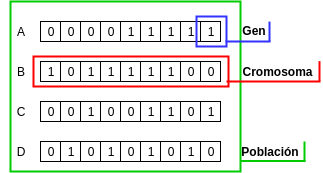
\includegraphics[width=0.6\textwidth,height=5cm]{Imagenes/PoblacionGA}
    \caption{Ejemplo de estructura de población, cromosomas y genes.}
    \label{fig:figuraPoblacionGA}
\end{figure}

Un algoritmo genético comienza con una \textit{población inicial} de cromosomas, generados de forma aleatoria, que representan la primera generación de posibles soluciones. A continuación,
se evalúa cada cromosoma de dicha población mediante la función fitness para comprobar cómo de bien resuelve el problema planteado. Al finalizar, cada candidato tiene asignada una puntuación
de fitness que representa lo bien (o lo mal) que lo ha hecho intentando resolver el problema.
Una vez con la población inidical completamente evaluada, el \textit{operador de selección} escoge de entre toda la población de candidatos algunos cromosomas para la reproducción (creación
de una nueva generación). Existen muchos tipos de algoritmos de selección, pero generalmente en todos ellos se eligen los cromosomas que mejor puntuación fitness han obtenido, buscando que
las siguientes generaciones creadas a partir de ellos den resultados como mínimo igual de buenos a los suyos.
En el siguiente paso, el \textit{operador de recombinación} simula las operaciones de recombinación de cromosomas presentes en las operaciones de división celular de tipo \textit{meiosis}. En la figura
\ref{fig:figuraCrossover} se puede observar un ejemplo de operación de recombinación. En este proceso se seleccionan dos cromosomas de la población y se recombinan para crear dos descendientes.

\begin{figure}[H]
    \centering
    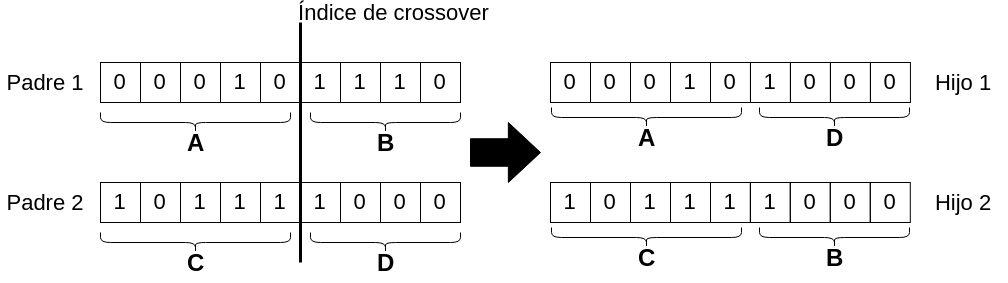
\includegraphics[width=1.0\textwidth,height=5cm]{Imagenes/CrossoverExample}
    \caption{Ejemplo de operación de recombinación de dos cromosomas.}
    \label{fig:figuraCrossover}
\end{figure}

El \textit{operador de mutación} modifica de forma aleatoria genes de los cromosomas descendientes (por ejemplo cambiando un 1 por un 0 y viceversa, en cromosomas binarios). Estas mutaciones ocurren
generalmente con una probabilidad bastante baja. A primera vista, el proceso de mutación puede parecer inecesario e incluso entorpecedor. La realidad es que toma un papel muy importante. Las operaciones
de selección y recombinación mantienen la información genética de los cromosomas con mejor puntuación fitness, pero estos cromosomos sólo son considerados los mejores respecto a la población de la generación
en la que fueron elegidos. Esto puede provocar que el algoritmo converga demasiado rápido y de una solución final alejada de la solución máxima. En otras palabras, puede provocar que el algoritmo se quede
atascado en un máximo local antes de encontrar el máximo global óptimo. El operador de mutación ayuda a proteger el algoritmo de este problema manteniendo la diversidad en la población, a costa de aumentar
el tiempo de convergencia.

Lo normal es que la selección, recombinación y mutación continuen hasta que el numero de descendientes es igual al número de cromosomas de la población inicial, para que esta segunda generación este compuesta
en su totalidad por descendentienes y reemplace a la población anterior.

Ahora la segunda generación se evalúa mediante la función fitness y todo el proceso se repite. Es una práctica comúm el almacenar el cromosoma con la mayor puntuación de fitness junto con dicha puntuación para
guardar un registro del mejor cromosoma hasta el momento.

Los algoritmos genéticos iteran hasta que la puntuación fitness del mejor cromosoma hasta el momento se estabiliza y no cambia en una serie de generaciones. Esto significa que el algoritmo ha convergido en una
o solución. A todo el proceso de iteraciones se llama \textit{carrera} (en inglés, \textit{run}). Al final de cada carrera se tiene, normalmente, al menos un cromosoma que es una solución lo suficientemente
buena (lo suficientemente \textit{fit}) del problema. Dependiendo del tipo de algoritmo utilizado, la mejor solución puede ser el mejor cromosoma que ha aparecido en todas las iteraciones o el mejor cromosoma
de la última generación.

El rendimiento de un algoritmo genético depende enormemente de los métodos utilizados para codificar posibles soluciones en cromosomas y el criterio utilizado en la función fitness para evaluar a los candidatos.
Otros detalles importantes a tener en cuenta son las probabilidades de recombinación y mutación, el tamaño de la población y el número de iteraciones. Estos valores puedes ser ajustados convenientemente después
de analizar el rendimiento del algoritmo tras unas carreras de prueba.

Los algoritmos genéticos tienen una gran variedad de aplicaciones. Algunos ejemplos destacados son la \textit{programación automática} y el \textit{"machine learning"}. Funcionan también especialmente bien para
modelar distintos fenómenos en economía, ecología, el sistema inmunológico humano, genética y sistemas sociales.
